Both the Halton sequence and the Hammersley point set use the radical
inverse function $\phi_b(i)$, where $b$ is a prime base and $i$ is
a nonnegative integer index, to generate samples.

We use Python to precompute the samples. First, we implement helper
methods for (i) computing the radical inverse given a prime base and
an index, and (ii) computing the next radical inverse incrementally.
We follow the pseudocode provided in the lecture slides
(\emph{Monte Carlo II}, slides~19--20).

\lstinputlisting[
    language=Python,
    firstline=1,
    lastline=31,
    firstnumber=1
]{code/4_2_radical_inverse.py}

\textbf{a) Halton sequence.}

Given the number of samples and a list of prime bases, we compute
the Halton samples iteratively. For the first point, we evaluate
the radical inverse directly for each base. For each subsequent
coordinates, we use the incremental radical inverse function.

\lstinputlisting[
    language=Python,
    firstline=1,
    lastline=12,
    firstnumber=1
]{code/4_2_sequence_generation.py}

\textbf{b) Hammersley point set.}

Unlike the Halton sequence, the Hammersley point
set uses $i/N$ as the first coordinate of each point:
\[
\mathbf{h}_i = \left(\frac{i}{N},\,\phi_2(i)\right),
\qquad i=0,\ldots,N-1.
\]
Here, $N=2^n$ is the total number of points, and $n$ is an integer
exponent. The subsequent points are computed the same as in Halton sequence.

\lstinputlisting[
    language=Python,
    firstline=14,
    lastline=25,
    firstnumber=14
]{code/4_2_sequence_generation.py}

\begin{figure}[htbp]
    \centering
    \begin{minipage}[t]{0.48\textwidth}
        \centering
        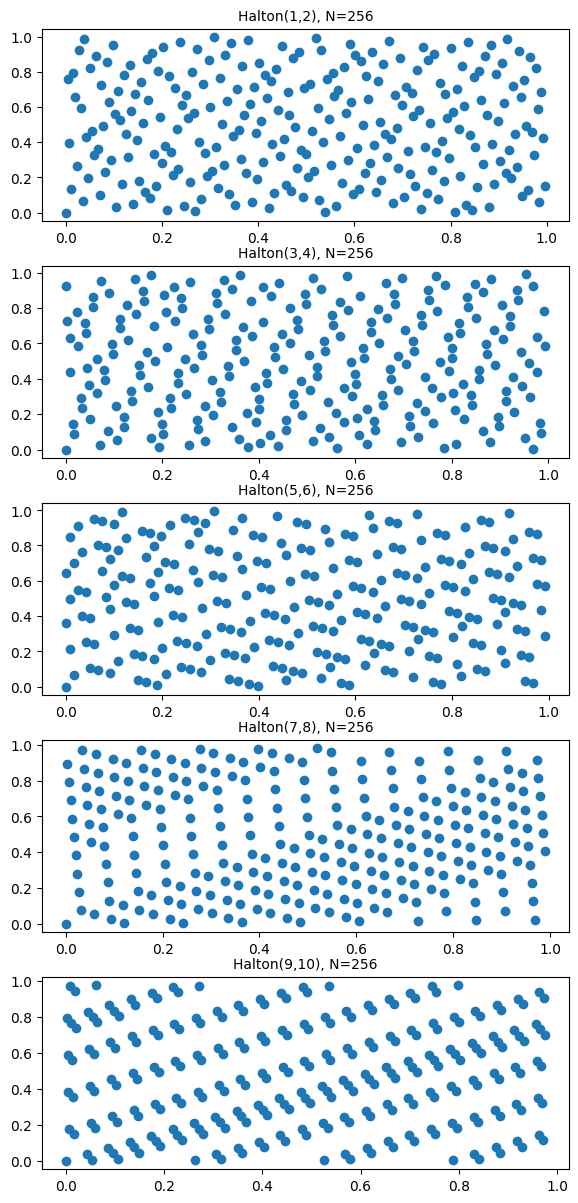
\includegraphics[width=\linewidth]{pictures/halton.png}
        \par\small (a) Halton sequences
    \end{minipage}
    \hfill
    \begin{minipage}[t]{0.48\textwidth}
        \centering
        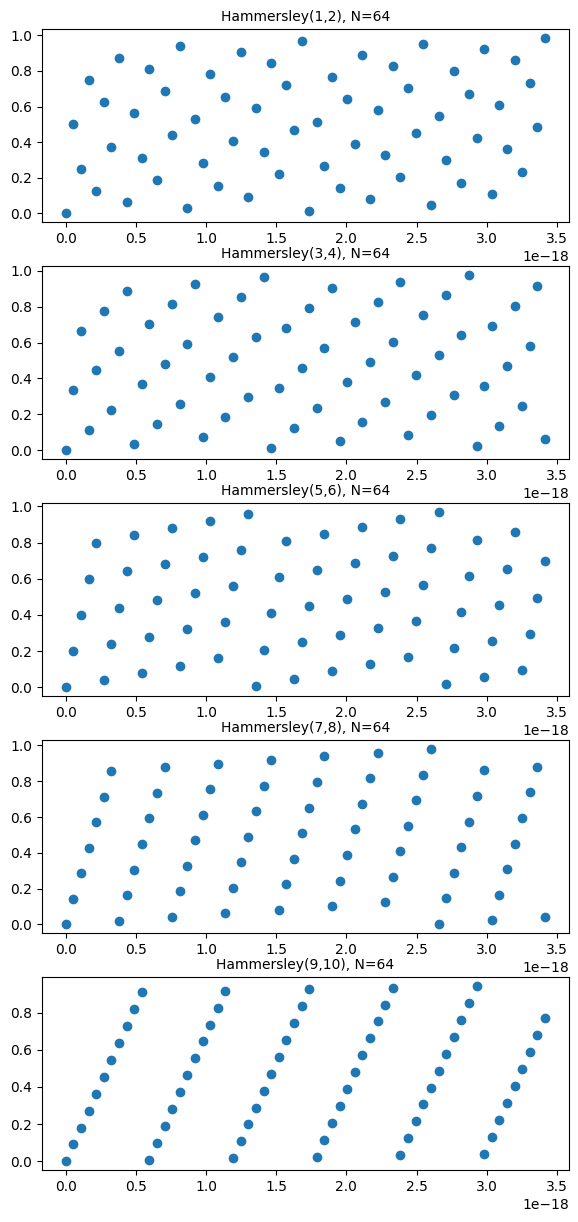
\includegraphics[width=\linewidth]{pictures/hammersley.png}
        \par\small (b) Hammersley point set
    \end{minipage}
    \caption{Sample distributions generated using the Halton sequence
    and the Hammersley point set.}
    \label{fig:halton-hammersley}
\end{figure}

\textbf{c) Bitwise radical inverse.}

For base $2$, we compute the radical inverse using bit operations.
At each iteration, we extract the least significant bit of the
index and append it to the reversed integer. We then shift the
index one bit to the right and double the denominator.

After processing $k$ bits, dividing the reversed integer by $2^k$
gives $\phi_2(i)$.

\lstinputlisting[
    language=Python,
    firstline=1,
    lastline=10,
    firstnumber=1
]{code/4_2_binary_radical_inverse.py}
